% Formatting for JEcol

\documentclass[12pt]{article}

% amsmath package, useful for mathematical formulas
\usepackage{amsmath}
% amssymb package, useful for mathematical symbols
\usepackage{amssymb}

% graphicx package, useful for including eps and pdf graphics
% include graphics with the com and \includegraphics
\usepackage{graphicx}

% citep package, to clean up citations in the main text. Do not remove.
\usepackage{natbib}

\usepackage{color} 

\usepackage{multirow}

\usepackage{xcolor} % Required for specifying colors by name
\definecolor{color}{RGB}{128,0,0} % Define the color used for highlighting throughout the book
\definecolor{blue}{RGB}{69,74,159} %Redifines the default for the color blue
\definecolor{color}{RGB}{0,0,0}%{64,63,111} %navy blue % Define the color used for highlighting throughout the book
\definecolor{blue}{RGB}{69,74,159} %Redifines the default for the color blue
\definecolor{niche}{RGB}{202, 0, 32}
\definecolor{neutral}{RGB}{4,4,160}
\definecolor{nineu}{RGB}{245,219,58}
\definecolor{grey}{RGB}{180,177,172}

\usepackage{makecell} % for cell alignment 

\usepackage{mdframed} % for cell alignment 

% Use doublespacing - comment out for single spacing
\usepackage{setspace} 
\doublespacing

% Text layout
\topmargin 0.0cm
\oddsidemargin 0.5cm
\evensidemargin 0.5cm
\textwidth 16cm 
\textheight 21cm

% Bold the 'Fig #' in the caption and separate it with a period
% Captions will be left justified
\usepackage[labelfont=bf,
labelsep=period,justification=raggedright]{caption}
\renewcommand{\figurename}{Figure}

% Leave date blank
\date{}

\pagestyle{myheadings}
%% ** EDIT HERE **
\usepackage{lineno}
\linenumbers

%% ** EDIT HERE **
%% PLEASE INCLUDE ALL MACROS BELOW

%% END MACROS SECTION

\begin{document}

\begin{flushleft}
{\Large
{\textbf{Tailoring species abundance distributions with
trait-environment correlations}}
}
\end{flushleft}


% abstract 150 words
\section*{Abstract}

%short abstract
%We propose a novel, general test to assess which mechanisms drive SADs. It translates niche and neutral mechanisms into fixed and random effects in a generalized linear mixed model. We applied this methodology to fern metacommunity along an altitudinal gradient. Hypotheses for niche processes, neutral and an hierarchical combination of both were tested. We found that although some ecological strategies confer on average more abundance in a particular altitude, drift results in variance in species abundances within the same ecological strategy. Accordingly, we were able to define ecological strategies in fern community based on synthetic and objective traits, and our modeling approach unpack neutrality in drift and limited dispersal mechanisms. Furthermore, predictions from our model fit SADs on each altitude. By adding information of species traits we did not reject the idea of functional equivalence of species, we delimited the influence of neutral processes on community assembly and SADs. 

% long abstract: 
%The pattern of few abundant and several rare species is considered a general law in ecology. Since both niche and neutral models can explain species abundances distributions (SADs), incorporating species differences in relation to its traits can help us understand to what extent functional divergence and equivalence can affect SADs. We used a trait-environment approach to understand which ecological strategies of species, if any, affect SADs in a fern metacommunity along three mountain ranges in a Brazilian Atlantic rainforest. We tested hypothesis simultaneously for purely neutral, purely niche and an hiearchical combination of both processes (emergent group, i.e. combination of groups of species defined by functional divergence that within behave as functional equivalents). We built statistical models using generalized linear mixed models (glmm) to represent our hypothesis. Our framework is based on the idea that we can translate neutral and niche processes into random and fixed effects in glmm's. We modeled the effect of dispersal limitation and drift within species sharing the same ecological stategy as random effects and used fixed effects to represent niche influences due to species ecological strategies and the altitudinal gradient. We found that species abundances are defined by a hierarchical combination of niche and neutral processes. We identified that combination of different states of laminar thickness and life form defines an ecological strategy and the emergent group. Although some ecological strategies are related to high abundance values in a particular altitudinal level, we still found a variance component in abundance among fern species sharing the same ecological strategy. Variance was explained by random effects representing functional equivalence within species sharing the same ecological strategy and limited dispersal among altitudinal levels and mountain ranges. Tradeoffs of an ecological startegy with its position on the gradient are due to strategies for reducing water loss across the altitudinal gradient. Additionally, we found that abundance predicted by our model fits perfectly with SADs on each altitudinal level. Finally, on the niche side, we defined ecological strategies in fern community based on synthetic and objective traits. On the neutral side, our modelling approach unpack neutrality in drift and limited dispersal mechanisms. By adding information of species traits we do not rejected the idea of functional equivalence of species, we refined the scope of the effect of neutral processes in terms of drift within emergent groups and limited dispersal.

%JEcol abstract

1. Given that both niche and neutral models can explain species abundances distributions (SADs), incorporating species differences in relation to its traits can help us understand to what extent functional divergence and equivalence can affect SADs. We proposed a trait-environment approach to understand which ecological strategies of species, if any, affect SADs at metacommunities across environmental gradients. 

2. We propose a straightforward framework to simultaneously test hypothesis for purely neutral, purely niche and and a hierarchical combination of both processes (i.e. combinations of groups of species that are functionally divergent across groups but neutral within the group). This framework combines functional traits with generalized linear mixed models (GLMMs) to represent the niche and neutral processes. Specifically, we show how to translate neutral and niche processes into random and fixed effects in GLMM's. For neutral processes we show how our framework can separate dispersal limitation and drift.

3. We used this framework to understand which ecological strategies of species, if any, affect SADs in a fern metacommunity along three mountain ranges in a Brazilian Atlantic rainforest. We found that a hierarchical combination of niche and neutral processes best explained the data. Different combinations of laminar thickness and life form define distinct ecological strategies. Specific ecological strategies determined high abundances at a given latitude, consistent with the idea of ecological filtering, but we also found a variance component in abundance among fern species sharing the same ecological strategy. This variance in abundance within a group was explained by a combination of drift and dispersal limitation. Tradeoffs of an ecological strategy with its position on the gradient are due to strategies for reducing water loss across the altitudinal gradient.

4. As demonstrated by our example, our framework has the potential to advance the goal of quantifying the relative importance of different processes (niches/filtering, drift, and dispersal limitation) from spatially structured abundance and functional trait data. Additionally, our framework allowed us not only to rebuild SADs curves for local communities, but also to provide a mechanistic explanation for species abundance patterns. 

%Tweetable abstract
%We present a framework to tailor species abundances in local communities by untying the effect of niche and neutral process.

%Why at JEcol
%We present a simple linear modeling framework to reveal the influence of niche and neutrality on community assembly. Besides its generality, our framework shows quantitatively the influence of both processes. 

{\bf Keywords}: emergent groups, drift, fern communities, functional groups, limited dispersal, neutrality, niche, SADs.

\newpage

\section*{Introduction}

Most species abundance distributions (SADs) in biological communities can be explained equally well by niche and neutral mechanisms \citep{McGill2007}. In this case, the problem of distinct processes explaining the same pattern seems to be related to the fact that SADs do not use species identities, which is indeed consistent with the idea of ecological equivalence in neutral theory. Ecological equivalence implies that trophically similar species are demographically identical \citep{Hubbell2001, Hubbell2005}. Therefore, differences in species abundances should be a result of random birth and death events at local scale that make communities diverge by drift if dispersion is limited \citep{Hubbell2001, Hubbell2005}. 
In contrast with this neutral view, species identities would matter if the lineages evolved a distinctive set of adaptive traits that translate into different niches. In the latter case species traits should correlate with abundances, and thus one way to distinguish between neutral and niche processes on SADs would be to assess such correlations. 
If the ecological equivalence hypothesis is rejected, a strong theory for SADs would be the one that could predict not only the shape of the curve but also if a species would be common or rare based on its traits \citep{Mcgill2003}.
For instance, SADs were described as a mixture of abundances of two groups of species, the core (persistent) and satellite (occasional) species \citep{Magurran2003}. Furthermore, \cite{Supp2015} showed that core and satellite species exhibit different life-history strategies, showing a link between temporal persistence, local abundance and species life-history traits.

The recognition of different groups of species in the local community is an important step to put SADs in a broader ecological and evolutionary context \citep{McGill2007, Swenson2012}, but we can go further by asking what defines each group. The obvious choice to identify groups of species in SADs is to look for traits that correlate with their abundances. Thus, placing SADs in a framework that allows to test the ecological equivalence of species would help disentangling niche and neutral mechanisms in predicting species abundances in a community. Assessing trait-environment correlations in community ecology has concerned ecologists for decades since \cite{Raunkiaer1934} characterization of plant life forms adapted to the environment \citep[see also][]{Grime1977, Connell1978}. Early development of trait-based approach focused on descriptions of variation of life history traits along environmental gradients. In the past 20 years trait-based approaches focused on quantitative measurements of traits for testing non-random trait dispersion in community assembly
\citep{Swenson2012}. The redefinition of the niche concept \citep{Chase2003}, the modern coexistence theory \citep{Chesson2000}, and Hubbell's proposal of neutral theory \citep{Hubbell2001} contributed to the bloom of functional ecology as a test against neutral theories. Empirical and theoretical tests in the context of functional ecology have been followed by a massive analytical development \citep{Kraft2010} from basic functional diversity measures
\citep{Petchey2002a, Petchey2007} to different approaches for incorporating functional evenness and divergence \citep{Mason2005, Pavoine2009} and multi-trait analysis \citep{Laliberte2010}, patterns of niche overlap \citep{Mason2008}, mechanisms of environmental filtering \citep{Kraft2007, Mayfield2009}, and trait
variation across environmental gradients \citep{shipley2006plant, cornwell2009community, messier2010traits}. 
The remarkable influence of trait-based approaches in plant community ecology could be considered a paradigm shift from species to trait-based ecology \citep{Pavoine2011, Swenson2012}, represented by the emergence of methods and theories as well as the implementation of a global database for plant species traits (TRY) \citep{Kattage2011}. Still, much of the trait-based approach focused on species interactions independent of SADs \citep{Swenson2012}. 
Even though there are some efforts of incorporating trait information in SADs \citep{Magurran2003, Supp2015} we can still go further not only asking what defines functional groups in SADs but also what is the relative importance of biological traits versus stochasticity on shaping species abundances. 
 
There is an emerging consensus that both niche and neutral processes are important for community assembly \citep{Vellend2014} and that community ecology should advance on how the two processes operate together \citep{Gravel2006, Herault2007}. One way of combining neutral and niche processes should be through the delimitation 
of the set of species in which neutrality applies \citep{Tilman2004, Scheffer2006, Herault2007, Holt2007}. Emergent Groups are defined as sets of species in a local community which are functionally similar enough with each other that they dynamics is well approximated by neutral theory \citep{Herault2007}. Thus, niche differentiation defines each Emergent Group, and within the Emergent Group neutrality defines species abundances in the local community. The Emergent Group approach represents the scenario in which neutral and niche processes operate at different levels generating SADs. Herein, we propose a framework to quantify the influence of neutral and niche processes at local and regional communities.  

Our main goal is to test which mechanisms, in a hierarchy from neutral to niche models, drive species abundances in local communities along environmental gradients. We used as a study system metacommunities of ferns across an altitudinal gradient sampled in three localities. 
We start from three potential mechanisms that can explain SADs: (i) purely neutral,  (ii) purely niche, (iii) the integration of both with the Emergent Group approach, and derived four hypotheses.
The first hypothesis is that neutral processes prevail and species abundances vary among communities randomly, as a result of drift under limited dispersal.
Our second hypothesis is that niche processes prevail and species abundances are determined by a set of adaptive traits, which we call an ecological strategy. 
In this case, species abundances in the local community would be a result of dissimilarities in ecological strategies of species.
Also, SADs can change because the optimal strategy can vary along the environmental gradient. 
Third, species abundances are defined by a combination of niche and neutral processes through Emergent Groups. In the third scenario, ecological strategies of species affect abundance but ecological drift ensues random differences of species abundances within each group. As in the niche scenario, the success of the ecological strategies can depend on the environment.
Fourth, assuming that neutrality effects can appear not only as drift within Emergent Groups, we hypothesize that processes generating Emergent Groups could occur combined with limited dispersal. 
We show how these hypotheses can be translated into fixed and random effects in linear mixed models.
We thus propose a novel approach that uses random structure of mixed models to represent
drift and limited dispersal in the hypotheses where neutrality operates.  Finally, we confronted all hypotheses simultaneously using a model selection framework 
to test the corresponding models of species abundances.

\section*{Material and methods}

\subsection*{Study site and sampling methods}
In order to test for trait-environment correlations on species abundances we 
used abundance data of fern species sampled along an
altitudinal gradient  in three  
locations of the Brazilian Atlantic rainforest at 
Serra
do Mar mountain chain, in Paran\'a State from \cite{Paciencia2008}.
The sampled gradient ranged from
sand dune vegetation at the coastal plain (0 to 10 m a.s.l.) to high montane 
Ombrophilous Forest areas (1,500 m a.s.l.) in three mountain ranges 
in this ecorregion: 
Serra da 
Graciosa (25{$^{\circ}$} 21'S, 48{$^{\circ}$} 54'W), Pico do Marumbi 
(25{$^{\circ}$} 27'S, 48{$^{\circ}$} 55'W), and Serra da Prata (25{$^{\circ}$} 
37'S, 48{$^{\circ}$} 41'W). From 0 to 700 m a.s.l. the climate is subtropical with hot summer and 
without dry season (Cfa) and with mean temperature 
during summer above 22{$^{\circ}$} C. Above 700 m a.s.l. the climate is 
subtropical with warm summer and without dry season (Cfb). Since all mountains 
are part of the same mountain chain, with controlled distance (from 14 to 41 km 
distant from each other), we considered sampling sites at the same
altitudinal level as replicates from local communities. 
In fact, floristic similarity among sites at the same altitude is higher than 
floristic similarity among sites at the same mountain range 
\citep{Paciencia2008}. 
 
Vegetation along the altitudinal gradient varies following changes of soil, 
humidity, temperature, and precipitation levels. 
The coastal plain is occupied by scrubland and low forest on poor, white-sand 
soils. 
Lowland Ombrophilous Forest occupy the transition between the coastal plain and 
the mountain range, where the sandy soil has poor drainage but higher fertility. 
Submontane Ombrophilous Forest occurs from 30 to 400 m a.s.l. and harbors large 
trees growing on deep clay soils of the hillside. Montane Ombrophilous Forest occurs 
from 400 to 1,000 m a.s.l. on lithic soils limiting the growth of large 
trees. Montane forests occur where there are less severe environmental 
conditions in terms of humidity, temperature, and precipitation. High-montane 
Ombrophilous Forests occurs from 1,000 to 1,600 m a.s.l. with predominance of 
lithic soils and where woody stractum is composed by crooked trunks of small 
size. 
We used elevation above sea level to represent the altitudinal gradient as a
proxy for variation in vegetation type, humidity, temperature, and
precipitation.  
Although altitude represents a set of variables, it is 
recognized that
fern species have specific elevational distributions related to their
ecological requirements \citep{Mehltreter2010} and fern diversity is correlated with elevation 
exhibiting a peak at intermediate elevations \citep{Kessler2001,Cardelus2006,WatkinsJr2006}. 

A total of 30 sites were sampled, 10 in each locality,
distributed at 0, 10, 50 m, and from 200 to 1,400 at 200 m elevation
intervals. In each site, one 20 x 20 m plot was settled. 
All fern individuals under 2 m from the forest floor were sampled, being
included terrestrial ferns, such as terrestrial herbs and tree ferns,
hemiepiphyte and epiphyte herbs (only individuals in which the lowermost leaf was up to 2 m from the ground). 
Abundance was measured as the number
of ramets of each species in each sample unit. The study of Paciencia (2008) 
recorded
19,938 individuals belonging to 155 fern species. 

\subsection*{Ecological strategy and species abundances}
In order to assess trait-environment correlations with species abundances we tested which set of traits define an ecological strategy. We chose three traits
that are related to species local abundances and that 
should respond to environmental changes 
along the altitudinal gradient. 
Our choice was based on limitations imposed on ferns due to aspects of
their biology such as intolerance to fluctuating conditions and poorly
controlled evaporative control \citep{Page2002}. Ferns may be less efficient in 
water use than seed plants due to an inefficient stomatal control, that rely 
only on passive closure \citep{Brodribb2011}. 
In the absence of
strategies to deal with such limitations, ferns have more success on
moist habitats where environmental conditions remain constant
\citep{Page2002}, characteristics such as those found in intermediate altitudes 
of the studied gradient.
In fact, in the context of Emergent Groups, species traits involved in potential 
challenges faced by plants should be good candidates for delineating Emergent Groups 
\citep{Herault2007}.

We chose two basic
leaf traits that can confer advantages on dealing with water limitations:
thickness and presence of 
indumentum (Table \ref{trait}). Thick leaves can store water 
and increase water use efficiency and the presence of indumentum can reduce 
water loss from evapotranspiration \citep{Watkins2012}. Thus, thick and/or
indumented leaves may enable species to persist on harsh environments
such as lowland or high montane forests. 
Additionally, life form, defined by the subtract
a species occupies (e.g., terrestrial, hemiepiphyte, and epiphyte), is an important
niche dimension in fern communities segregating species
occupying different substrates. 
Based on the assumption that species within a life form may interact
more intensely we included species life form as another trait to define an 
ecological strategy. We then classified all 155 species based on its traits (see Table S1 in Supporting Information). 



\subsection*{Model fitting and selection}

To assess the influence of species traits and the environmental gradient on species abundances we translated the niche, neutral and emergent group hypotheses in generalized linear models (GLM) and generalized mixed-effect models (GLMMs). 
For all models, we used as response variable species abundance recorded at each site and thus absences were accounted as zeros. 

To test our hypotheses we built 35 models representing each of our general hypotheses (Box 1 and Table \ref{mod}).
Models corresponding to the idiosyncratic, neutral dynamic, Emergent Groups, and Emergent Groups with limited dispersal hypotheses were built using GLMM approach. Each term in the models represent a particular process. Models corresponding to purely niche effects were built using GLMs. We assumed that neutrality within Emergent Groups, limited dispersal and ecological drift can be expressed as a random factor in the GLMMs since we are incorporating random variation of abundance from the overall mean value in a particular level. 
Species abundances were modeled as a Poisson variable with a logarithm link function. 
In our case, the effect of the environmental gradient is represented by altitude which is expressed as a fixed effect in niche and Emergent Groups models
and included as a second-order polynomial, since the study of \cite{Paciencia2008} detected 
unimodal relationships of abundances with the altitudinal gradient.
Niche theory predicts that differences in species abundances should be due to differences in species traits in response to the environment. Therefore, the use of ecological strategies as fixed effects means that species sharing the same ecological strategy would have the same linear response in terms of abundance along the altitudinal gradient. In contrast, in a neutral community abundances of all species drift randomly around the same mean value. If so, abundance of each species would be a realization of the same random process, which would translate into a random effect of species identities in a linear model. 
We translated the effect of drift under limited dispersal as a random effect of species identities restricted 
between metacommunites (e.g., regional communities at different mountain ranges) and within metacommunites (e.g., local communities at different elevations) representing low means of movement of individuals across space.

Confronting a set of statistical models can be done using model selection by identifying which prediction the data support best. By combining model selection with the translation of each hypothesis in a set of models, we can have models that express alternative hypotheses and then compare them simultaneously \citep{Johnson2004}.
As a result, based on the selected model we can predict the abundance of a species along the environmental gradient and identify which factors best predicts species abundance rank and, thus, which class of mechanisms prevail in the 
assemblage of the community. 
Therefore, we used GLMs and GLMMs as a way to build strong inferences (sensu \cite{Mcgill2003}) on the influence of ecological strategies and altitude on species abundances. 
By using model selection with GLM and GLMMs we were able to translate alternative hypotheses in competing models. 
GLMMs have been widely used in Ecology and Evolution since it is common to have non-normal biological data that involves random effects \citep{Bolker2009}. Here, we inovated by using the random structure of mixed models to represent alternative hypotheses involving neutral processes such as drift and limited dispersal. 


\global\mdfdefinestyle{exampledefault}{%
linecolor=black,linewidth=1.5pt,%
leftmargin=.01cm,rightmargin=.01cm
}

\begin{mdframed}[style=exampledefault]
\newpage
\begin{singlespacing}
 \textbf{Box 1. Predictions for each general hypothesis.} \\
 \noindent\rule[0.5ex]{\linewidth}{1pt}
  \paragraph{{\color{grey}{$\blacksquare$}} Idiosyncratic} ~\\ Differences in abundance are due random variation among communities and species.
\paragraph{{\color{neutral}{$\blacksquare$}} Neutral dynamic} ~\\ Differences in species abundances are due to limited dispersal (i) among metacommunities or (ii) among and within metacommunites. Therefore, local SADs are the result of random variation of abundances at each locality or sampling site, or both. %site and also SADs vary randomly among sites and localities. (ii) Differences in species abundances are due to limited dispersal among localities: same as above but random variation SADs do not vary among sampling sites within the same locality. 
\paragraph{{\color{niche}{$\blacksquare$}} Niche} ~\\ (i) Absolute fitness differences among strategies: the ecological strategy of a species affect species abundances but does not depend on the environment. (ii) Trait-environment correlation: the effect of ecological strategies on abundance are positive in some portions of the gradient but negative in others. 
\paragraph{{\color{nineu}{$\blacksquare$}} Emergent Groups} ~\\ (i) Absolute fitness differences among strategies, but there is random variation in species abundances among species sharing the same ecological strategy. (ii) Trait-environment correlation but there is stochastic differences in species abundances among species with the same ecological strategy.
\paragraph{{\color{nineu}{$\blacksquare$}} Emergent Groups with limited dispersal} ~\\ (i) Emergent groups with absolute fitness differences with limited dispersal: 
abundances are affected by ecological strategies but also have a random variation among species. This variation among species also occurs among metacommunites. 
(ii) Emergent groups model with limited dispersal among and within metacommunites. %and : 
Same as latter but with random variation on regional and local scales.  
(iii) Emergent groups model with trait-environment correlation and with limited dispersal at regional and local scales. Random variation among species also occur among and within metacommunities.
(iv) Emergent groups model with trait-environment correlation and with limited dispersal among metacommunities. 

\end{singlespacing}

\end{mdframed}

Model fitting was done using numerical routines to approximate maximum
likelihood \citep{Bates2013}. The models were then compared using the
Akaike Information Criteria (AIC), a measure of support by the data. 
The model with lowest AIC value was selected as the most plausible
statistical hypothesis and models with {$\Delta$}AIC differences less
than two were considered equally plausible. We reported marginal and conditional R${^2}$ \citep{Nakagawa2013} for the best model. Marginal R${^2}$ stands for variance explained by fixed effects, which in our framework can be interpreted as the variance explained by niche effects, whereas conditional R${^2}$ stands for variance explained by fixed and random effects, which in our framework represents the effects of niche and neutral effects.  
Data analysis was done on R software \citep{RCoreDevelopmentTeam2009}, using the packages lme4 \citep{Bates2013}.

\subsection*{Generating SADs}

In order to identify the effects of ecological strategies on SADs, for each altitudinal level, we built rank-abundance diagrams using the mean relative abundance of each rank among the mountain ranges. We then compared these empirical
values to the rank-abundances diagrams of the abundances predicted by the selected model at each site (i.e., local community). 

\section*{Results}

\subsection*{Neutral dynamic, niche, and Emergent Groups}

For our study system, we observed that species traits affect species abundance and interact with altitude, but
we still detected the effect of Emergent Groups and limited dispersal.
The best model have the effects of ecological strategy interacting with altitude and also the effects of
neutral drift within localities and sampled sites 
(Table \ref{pesos}, see also Tables S2 and S3).
It is worth noting that the set of models that express the Emergent Group and limited dispersal hypotheses accumulated almost all the evidence weight (sum of Akaike weight=0.99, with the weight of 0.96 for the best model). Also, most of the variance in abundance is explained by the combination of fixed and random effects (i.e. conditional R${^2}$), instead of fixed effects alone (conditional R${^2}$=0.85, marginal R${^2}$=0.09).  
In the selected model Emergent Groups were defined by combinations of
life form and leaf thickness:  
The selected model retain  as fixed effect life form and leaf thickness expressing different ecological strategies such as:
(i) terrestrial species with membraceous leaves; 
(ii) terrestrial species with coriaceous leaves;
(iii) hemiepiphyte species membraceous leaves;
(iv) hemiepiphyte species coriaceous leaves;
(v) epiphyte species with membraceous leaves;
(vi) epiphyte species with coriaceous leaves; as well as altitude and the interactions between altitude and ecological strategies. Since this model also retain species as the random effect, variation of abundance within ecological strategies represents the Emergent Groups. 

The interaction between strategy and altitude highlights that species
mean abundances within some combination of traits are higher in some
altitudinal levels but lower in others (Fig. \ref{grad}). 
Individuals of terrestrial and hemiepiphyte species with
membranaceous leaves present an abundance peak at intermediate
altitudes of the gradient (600 to 800 m). Individuals with coriaceous
leaves present higher values of abundance on  lowland forests, with
decreasing abundance values following the decrease in altitude (Fig.
\ref{grad}a-d). Whereas terrestrial and hemiepipyte species presented
similar patterns of abundance along altitudinal variation, we observed
a distinct pattern for epiphyte species. In general, epiphyte species
tended to be more abundant on extreme altitudes of the gradient (Fig.
\ref{grad}e-f). The pattern is more conspicuous for epiphyte species
with coriaceous leaves. It is remarkable that above 1,200 m epiphyte
species are predominantly abundant.
Although some combination of traits confer, on average, high values of abundance depending on the altitude, 
there was wide variation among abundances of species of the same Emergent Group as shown by wide
standard errors. The standard errors of predicted values matched %these
this
variation (Fig. \ref{grad}) which was captured by the interaction between random
effects of species with sites and with localities. In the model the interaction between species and localities accounted for random variation in abundances caused by drift under limited dispersal among metacommunities, whereas the interaction between species and localities accounted for variation in species abundance caused limited dispersal within metacommunites. 

Analyzing ecological strategies, we observe that for terrestrial and hemiepiphyte species individuals with membranaceous leaves present an abundance peak at intermediate altitudes of the gradient (600 to 800 m). Individuals with coriaceous leaves present higher values of abundance on  lowland forests, with decreasing abundance values following the decrease in altitude (Fig \ref{grad}.a-d). Whereas terrestrial and hemiepipyte species presented similar patterns of abundance along altitudinal variation, we observed a distinct pattern for epiphyte species. In general, epiphyte species tend to be more abundant on extreme altitudes of the gradient (Fig \ref{grad}.e-f). The pattern is more conspicuous for epiphyte species with coriaceous leaves. It is worth noting that above 1,200 m epiphyte species are predominantly abundant.   %% Não seria melhor começar com estes dados empíricos?
Although some combination of traits confer, on average, high values of abundance depending on the altitude, 
the success of a species is also conditioned to random variation of abundance in species of the same emergent group and 
limited dispersal related to localities and sampled sites, represented by predicted standard errors (Fig \ref{grad}).

\subsection*{Generating SADs}

When analyzing the general pattern of SADs along the altitudinal
gradient we observed high dominance on extreme altitudes -- 
lowland and high montane forests -- and more  
evenness on intermediate
altitudes (Fig. \ref{sads}).
The selected model provided an excellent fit of observed
values of abundance on SADs across the gradient (Fig. \ref{sads}).
As shown by the selected  
model, SADs reveal that certain combination of traits are associated with
the changes of species abundances at along the environmental gradient.  
At sites ranging from 400 to 1,000 m a.s.l. most of abundant species
had membranaceous leaves, 
independently of the life form
(Fig. \ref{sads}e-h). In contrast, at lowest and highest
altitudes, species with coriaceous leaves were among the most
abundant recorded. 
Terrestrial species with coriaceous leaves were abundant from
0 to 200 m (Fig. \ref{sads}a-d) and from 400 to 1,000 m (Fig.
\ref{sads}e-h) terrestrial species with membranaceous leaves were
abundant. Additionally, from 10 to 1,000 m we always found a
hemiepiphyte species with membranaceous leaves among the three most
abundant species in the communities (Fig. \ref{sads}b-h). In
contrast, hemiepiphyte species with coriaceous leaves, are, generally,
among rare species at sites above 600 m (Fig. \ref{sads}g-j). It is
notable the occurrence of epiphyte species among the most
abundant species at sites above  1,000 m (Fig. \ref{sads}i-j), as well as the increasing
dominance of this life form at high altitudes.  
In summary, as predicted by the selected model, general patterns of
abundance among species that share the same combination of traits 
are associated, on average, with higher abundances depending on the
altitude. Although, abundances vary markedly among species that share
the same trait combination, which is consistent
with the prediction of the selected model including the random drift
within Emergent Groups.

\section*{Discussion}

Taking the example of our study system, if one would analyze only the SADs of fern the communities one would observe the remarkable change in dominance along the altitudinal gradient, that some ecological strategies are associated with high abundance values, and that there there is still great variance in abundance among species that
share the same ecological strategy.  
With our modeling approach we can not only predict the shape of the SADs depending on the environmental gradient but also the different niche and neutral mechanisms generating it. By our model we can predict the mean abundance of a species given its ecological strategies and its position on the altitudinal gradient, representing the niche effect (Figure \ref{final}a).
Still, remains variability that can be attributed to random drift, supporting the idea of Emergent Groups, and through random variation of species abundances among and within metacommunities (Figure \ref{final}b).   
We demonstrated that whereas the
ecological equivalence assumption does not apply, there is still
influence of neutral processes such as drift within Emergent Groups
and limited dispersal on community assembly.
Therefore, our model express the assembly of fern communities as combination of 
selection and drift \citep{Vellend2010}. The gradient acts as an environmental
filter exerting a selective force on which species and trait frequencies will succeed
in a given local environment \citep{Webb2010}. 
Alternatively, within each emergent group,
species may have recruitment differences due to stochastic colonization
rates or limited dispersal, generating stochastic changes in species
abundances \citep{Gravel2006, Weiher2011}.


\subsection*{Tailoring SADs with mixed models} 

By using mixed-effect models we could describe SADs of each local
community accurately as a combination
of SADs of different functional groups with random variation.
In our models, abundances of each species on samples are described as a
Poisson process. Species with different ecological strategies have
different mean predicted abundances at each point of the environmental
gradient. The random effects allow
mean abundances to vary among species and sites within each ecological
strategy % at each environment. 
The predicted SADs are then the
abundances predicted 
by all these fixed and random effects, that express niche and neutral
processes. %, respectively.
Therefore our model applies the  
decomposing of SADs based on species traits \citep{Magurran2003} in
the context of Emergent Groups \citep{Herault2007}.

The classic hollow curve pattern of the SADs is generated by differences in fitness among species and alternative strategies lead to negative skew \citep{Magurran2003}. 
Thus, random variation in species ranks on SADs for the same ecological strategy is due to random demographic rates and random placement of species in localities. 
The consequence for SADs is that random processes generate variation in negative skewness. \cite{Magurran2003} attributed the negative skew to niche subdivision, without having to invoke neutrality. On the other hand, according to neutral theory \citep{Hubbell2001} negative skew would be a result of community size and immigration rate. Our model makes an accurate prediction for SADs based on how niche and neutrality affect community assemblage and SAD empirical skewness.

Approaches based on
functional traits have been used to demonstrate the importance of
environmental  filtering  in  structuring  diverse  ecological
communities \citep{lavorel2002predicting, Baraloto2012}. Even with a
lot of methodological development in recent years it is not easy to
disentangle between trait versus neutral influences and methods fail
to detect the signature of processes such as dispersal
\citep{kembel2009disentangling}. 
Linear models with random effects associated to species is 
an effective tool to describe
joint responses of species groups to environmental
gradients \citep{Jackson2012, Brown2014}. We extended this idea 
 choosing effects that can be interpreted as outcomes of neutral dynamics and niche processes.
Our modeling approach 
decomposes the effects of
neutrality in drift and limited
dispersal mechanisms. Drift is depicted by random variation in
abundance among species that share the same ecological strategy, while
limited dispersal is depicted as random variations of abundance of each
species at different spatial scales: among and within metacommunites (i.e., sampling sites and mountain ranges in our case). 
Our method is analogous to a variance partitioning of environmental and spatial variables \citep{Gilbert2004a} that decouples neutral and niche processes into distance and environment components. The advantage of our framework is that each term in the model represent a particular process and through model selection one can identify which combination of processes better explain species abundance.
%, Chang2013}
Therefore, linear mixed-effect models provides a straightforward way to
translate hypotheses on the effects of niche, drift
and dispersal on species abundances in
competing statistical models. Information indexes like AIC can then be
used to express the support provided by data to each model \citep{Burham2002, Johnson2004}.
The simultaneous comparison of competing models that map
to alternative hypotheses grounded in the theory is the 'golden
standard' of model-based inference \citep{Hilborn1997} 
and a much-needed improvement to
phenomenological 'curve-fitting' to SADs \citep{Mcgill2003}.

\subsection*{Insights from the study system to niche and neutrality interplay}

We defined ecological strategies for fern
communities based on synthetic traits that are relevant for community
assembly. 
Laminar thickness and life forms are obvious traits for
plant ecologists that we can in fact relate with differences in species
abundances besides being. % comprising an objective criterion to define groups. 
Additionally,
they are important traits in an evolutionary context since one of the most important event
of fern diversification is attributed to the arise of strategies to cope with
new niche space and low-light and water requirements in angiosperm-dominated forests in Cretaceous and
Cenozoic periods. 
\citep{Schneider2004, Schuettpelz2009}.
Given that an ecological strategy predicts
different abundances depending on the position of the gradient that a
species is, we infer that there are tradeoffs on having some
ecological strategies. Having thick leaves, for instance, may be a
good
characteristic for dealing with more severe conditions in terms of
water availability -- on lowland forests and above 1,200 m -- as
predicted by our model, specially in the case of ferns that have
reduced water efficiency \citep{Page2002,
Watkins2012,Vasco2013}. However, having thick leaves on moist and
moderate environments do not result in more success in terms of local
abundances. 
Indeed conservative water use strategies of ferns seem to
constrain their utilization of light on low-light forests
\citep{Zhang2009}, representing a light use vs. water storage tradeoff.
Actually, as predicted by our model it is worth having thin leaves to
be successful in intermediate positions of the altitudinal
gradient. 

Our results also highlighted the importance of life form for the average
fitness of fern species.
Different predicted abundance values within the same ecological
strategy among life forms reinforces the assumption that terrestrial
and epiphyte ferns can have different physiological and life cycle
characteristics to deal with water and nutrient availability
\citep{Page2002, Watkins2012}. In general, epiphyte species 
deal better with limited water and nutrient sources than
terrestrial species \citep{Page2002, Schuettpelz2009,
Watkins2012}. This can explain why, in general, epiphyte species
despite of the leaf trait are more  
abundant on the
extremes of the gradient, specially on high altitudes. In addition to
leaf traits epiphyte fern species can also count with the gametophyte
traits to cope with low water availability since it seems
that epiphyte fern gametophytes are more resistant to survive on harsh
environments than terrestrial gametophytes \citep{Watkins2012}. 
Thus,
survival of gametophyte combined with sporophyte strategies can make
epiphyte species reach high values of abundance at 
 the extremes of the gradient. 
Alternatively,
terrestrial ferns have unique chemical compounds conferring advantage
on forest floor where there is low-light available \citep{Kawai2003}
and where species with thin leaves can succeed. Photoreceptors in terrestrial ferns
enhance light sensitivity by orienting leaves and chloroplasts and
have contributed to proliferation of ferns on low-light conditions
\citep{Kawai2003}. Having these compounds may offset strategies of
having thick leaves, contributing to high abundances of terrestrial
ferns on intermediate portions of the gradient, under dense canopy
cover. 
Again, there may be
a light use vs. water storage tradeoff for explaining why terrestrial
ferns with thicker leaves present higher abundance values only on the low
extreme of the gradient.  The biology of hemiepiphyte is still poorly
known in comparison with other life-forms
\citep{Watkins2012}. Nevertheless we identified an abundance pattern
different from epiphtyes with some similarities with terrestrial
species, supporting that hemiepiphyte species form a distinct
functional group.  There are few hemiepiphyte species with coriaceous
leaves, and those with membranaceous leaves are very abundant compared
to other life forms on intermediate altitudes.
Wherever hemiepiphyte with thin leaves occur,
mostly on the low to medium altitudes, they are very abundant, but
at highest positions of the gradient they do not occur.  Differently
from other studies on fern communities that separates the assemblage
into terrestrial and epiphyte components \citep{WatkinsJr2006,
Kluge2010}, our study identified hemiepiphyte species as a functional
group apart. Since most hemiepiphytes spend only part of its life
cycle as an epiphyte and can produce spores both on ground and on
trunks (JP pers. obs.), they can override terrestrial and
epiphytes abundances where they occur. 

Finally, in an historical context we can count three main strategies comprise
fern success: evolution of epiphytism, features that allow ferns
withstand dry conditions and a unique photoreceptor that enhanced fern
sensibility to light \citep{Schneider2004, Schuettpelz2009}. These life
history strategies of ferns that allowed them to persist and 
diversify on forest environments seem to be related to local ecological
strategies of species that can define the Emergent Groups in local
communities. 
The best supported models ascribed variation of abundances within
Emergent Groups to joint effect of drift, dispersal limitation, and environmental filtering independent of species traits.
Variance in species abundances are due to limited dispersal at a regional scale and habitat selection at a local scale. The fraction of environmental filtering not accounted for traits we incorporated in the model can be related to selection in the gametophyte generation.  
Since ferns are wind
dispersed plants it may be counterintuitive to consider that limited
dispersal can play an important role in community assembly. However,
it has been known that fern communities can be affected by limited dispersal \citep{Tuomisto2003c, Karst2005, Jones2006} in an ecological scale and 
it has been recognized that some groups of ferns present conspicuous
patterns of restricted speciation and diversification patterns driven
by dispersal limitation \citep{Korall2014, Labiak2014, Sundue2014} in an evolutionary scale. Since the limited dispersal is a stochastic component
in our model it seems reasonable to consider that limited dispersal is
randomly affecting spore dispersal at a regional scale and the local filtering can be related to variation in gametophyte establishment depending on the sampling site. Therefore, species are being limited regionally by a neutral process and locally by niche processes. 


\subsection*{Concluding remarks}

Rebuilding SADs from abundances predicted by our linear mixed model  
allowed us to understand how aspects of fern biology can influence community
patterns. We %%excluded the ecological equivalence assumption, and
identified the importance of tradeoffs on strategies for reducing
water loss across the altitudinal gradient. Among species with the
same strategy, we show that
neutral drift and limited dispersal among and within metacommunities also affect differences in
abundances.  
We proposed a mechanism that explains species
abundances in the community
combining neutral and niche-based
approaches. Hence, we simply refined the scope of neutral processes
affecting species abundances with the concepts of Emergent Groups and
limited dispersal. 
In this context, one promising question to be answered is
how ecological traits that define Emergent Groups at a particular community
evolved and how phylogenetic relatedness of species affects the
definition of the Emergent Groups. Placing Emergent Groups in an
evolutionary context may help understand integration levels of niche
and neutral processes in community assembly.

% Conclusions
Rebuilding SADs from abundances predicted by our linear mixed model  
allowed us to understand how aspects of biology of the study sytem can influence community
patterns. We %%excluded the ecological equivalence assumption, and
identified the importance of tradeoffs on strategies at the environmental gradient. Among species with the
same strategy, we show that
neutral drift and limited dispersal also explain differences in
abundances.  
One aspect worth noting is
that our modeling approach unpack neutrality in drift and limited
dispersal mechanisms. 
We proposed a mechanism that explains species
abundances in the community reconciling neutral and niche
approaches. Hence, we simply refined the scope of neutral processes
affecting species abundances in the context of emergent groups and
limited dispersal. Although we have applied our modeling approach to a specific data set, it comprises a general tool to disentangle niche and neural effects in any given community. 

\section*{Acknoledgments} 
Authors acknowledge Fundação O Boticário para Proteção da Natureza for facilitating the data collection. SM thanks CAPES DS for finacial support. Authors thanks Eduardo Santos and Luis Schiezari for insightful comments on previous versions of this manuscript. SM thanks to Brian McGill, Xiao Xiao and Sarah Supp for valuable discussions on the ideas presented in this manuscript. 

\section*{Authors' Contributions} 
SM, AAO and PIP performed conceptual modeling work, SM performed statistical analysis, MP, JP and PHL collected data and identified fern species, SM wrote the manuscript with all authors contributing substantially to the final version.

\section*{Data accessibility} 
All authors have agreed in putting data used in the manuscript available on Dryad.

\bibliography{besjournals}
\bibliographystyle{besjournals}

\newpage 


\section*{Tables}

% TABELA EM PÁGINA SEPARADA E NUMERADA ANTES DAS FIGURAS

\begin{table}[!hb]
    \caption{ Species traits included in the models to draw an ecological strategy.}\label{trait}
  %\rowcolors{1}{}{lightgray}
  \begin{tabular}{cp{4cm}p{6cm}}
\hline
\bf{Trait}	&	\bf{States}	&	\bf{Definition} 	\\
\hline
Laminar thickness	&	Membranaceous and coriaceous.	&	Laminar thickness was defined in a binary system in which species were separated in membranaceous (from membranaceous to papiraceous) and coriaceous (from cartaceous to coriaceous).	 \\
Indumentum	&	Absence and presence.	&	Defined as presence or absence of hair and scales on the laminar tissue.  \\
Life form	&	Terrestrial, epiphyte herb, and hemiepiphyte herb.	&	Species were classified in terms of habitat preferences for growth. Terrestrial life form includes terrestrial herbs and tree ferns. Epiphyte herbs were separated in epipyte and hemiepiphyte. \\
\hline
\end{tabular}
\end{table}


\newpage


\begin{table}[!ht]
  \caption{Fixed and random effects included in
each group of models. L=localities; SP=species; S=sampled sites, altitude as categorical variable or A=altitude as a second order polynomial; ES = ecological strategy, which is a factor with one level for each combination of traits observed in the species (see Table 2.1); {$|$}=conditioned to; {$*$}=interacting with.}\label{mod}
 \begin{center}
 
 \begin{tabular}{p{4cm}ccc}
 
\hline \bf General hypothesis	& \multicolumn{2}{c}{\bf{Effects}}	& {\bf Number of models} \\ 
	&		 \bf Fixed	&	\bf  Random	  & \\ \hline
\multirow{1}{4cm}{{\color{gray}{$\blacksquare$}} Idiosyncratic }	&		&	L{$+$}SP 	& 1 \\ %\hline
\multirow{1}{4cm}{{\color{neutral}{$\blacksquare$}} Neutral dynamic }&		& 1{$|$}SP+L{$|$}SP & 2	\\ 
&   & L{$|$}SP & \\ %\hline
\multirow{1}{4cm}{{\color{niche}{$\blacksquare$}} Niche	}&	ES	&	&  8	\\
	&	ES{$*$}A &		& \\ %\hline
\multirow{1}{4cm}{{\color{nineu}{$\blacksquare$}} Emergent Groups	} & ES	&	1{$|$}SP & 8	\\
	&	ES{$*$}A	&	1{$|$}SP &	\\ %\hline
\multirow{2}{4cm}{{\color{nineu}{$\blacksquare$}} Emergent Groups with limited dispersal}& ES & 1{$|$}SP+L{$|$}SP{$+$}S{$|$}SP & 16\\ 
& ES & 1{$|$}SP+L{$|$}SP & \\ 
&  ES{$*$}A & 1{$|$}SP+L{$|$}SP{$+$}S{$|$}SP & \\ 
 & ES{$*$}A & 1{$|$}SP+L{$|$}SP & \\ 
\hline
\end{tabular}
\end{center}
\end{table}


  \begin{table}[!ht]
  \caption{ Sum of Akaike weights for each general hypothesis, presented in descending order. For a complete table of model selection results consult Table S2. Best model representation: abundance ~ laminar thickness + life form + laminar thickness*altitude + life form*altitude + 1|species + localities|species + sampled sites|species (consult Table S3 for coeficient values.}\label{pesos}
  %\rowcolors{1}{}{lightgray}
  \begin{tabular}{p{4cm}p{6cm}cc}
   
\hline \bf General hypothesis	& \bf General prediction & \makecell{\bf Numbers \\ \bf of models} & \bf \makecell{Akaike \\ weights}	\\ \hline
Emergent Groups with limited dispersal & Emergent groups model with limited dispersal among localities and sampled sites  & 16 &  \makecell{0.9999 \\ (best model=0.9624)}\\  

Neutral dynamic	&	Differences in species abundances are due to limited dispersal 
among localities and sampled sites &	2 & {$<$}0.0001		\\ 

Emergent Groups	&	An ecological strategy influences abundance but there is 
stochastic differences in species abundances among species with the same 
ecological strategy, depending or not on altitude	& 8 &  {$<$}0.0001	\\ 

Idiosyncratic	&	Differences in abundance are due stochasticity among localities and 
species	 & 1	& {$<$}0.0001	\\ 

Niche	&	Ecological strategy of a species determines species abundances, depending or not on altitude	
& 8	& {$<$}0.0001		\\ \hline

\end{tabular}
\end{table}


\clearpage

\section*{Figures}

\begin{figure}[!h]
 %\begin{center}
%\includegraphics[scale=.75]{./fig1.pdf}
%\end{center}
\caption{Mean abundances of fern species (log) within each trait
    along the environmental gradient in a Brazilian Atlantic Rainforest of Paran\'a State. 
    Terrestrial individuals (A-B), Hemiepiphyte individuals
  (C-D), epiphyte individuals (E-F). Bars represent observed SE, solid lines represent abundance
  values predicted from the selected model and dashed lines represent predicted {$\pm$} SE.}\label{grad}
\end{figure}


\begin{figure}[!ht]
 \begin{center}
%\includegraphics[scale=.58]{./fig2.pdf}
\end{center}
\caption{Fern species relative abundance distributions (log) along the environmental gradient in a Brazilian Atlantic Rainforest of Paran\'a State. Dots represent mean abundance value among sampling sites at the same altitudinal level. Gray solid line represents predicted values by our best model for each altitude.}\label{sads}
\end{figure}

\begin{figure}[!ht]
 \begin{center}
%\includegraphics[scale=.48]{./fig3.pdf}
\end{center}
\caption{Interpretation of how niche and neutral processes can generate observed patterns of species abundances. (a) Environmental filtering selects the best ecological strategies of species depending on the environment. On average, the success of a particular ecological strategy is defined by niche. (b) Remaining variance of abundance is due to neutral processes such as drift among species sharing the same ecological strategies and limited dispersal among and within metacommunities.} \label{final}
\end{figure}

%% PI: nova figura com rad da metacomunidade, adicionada em 11/junho 2019
\begin{figure}[!ht]
 \begin{center}
%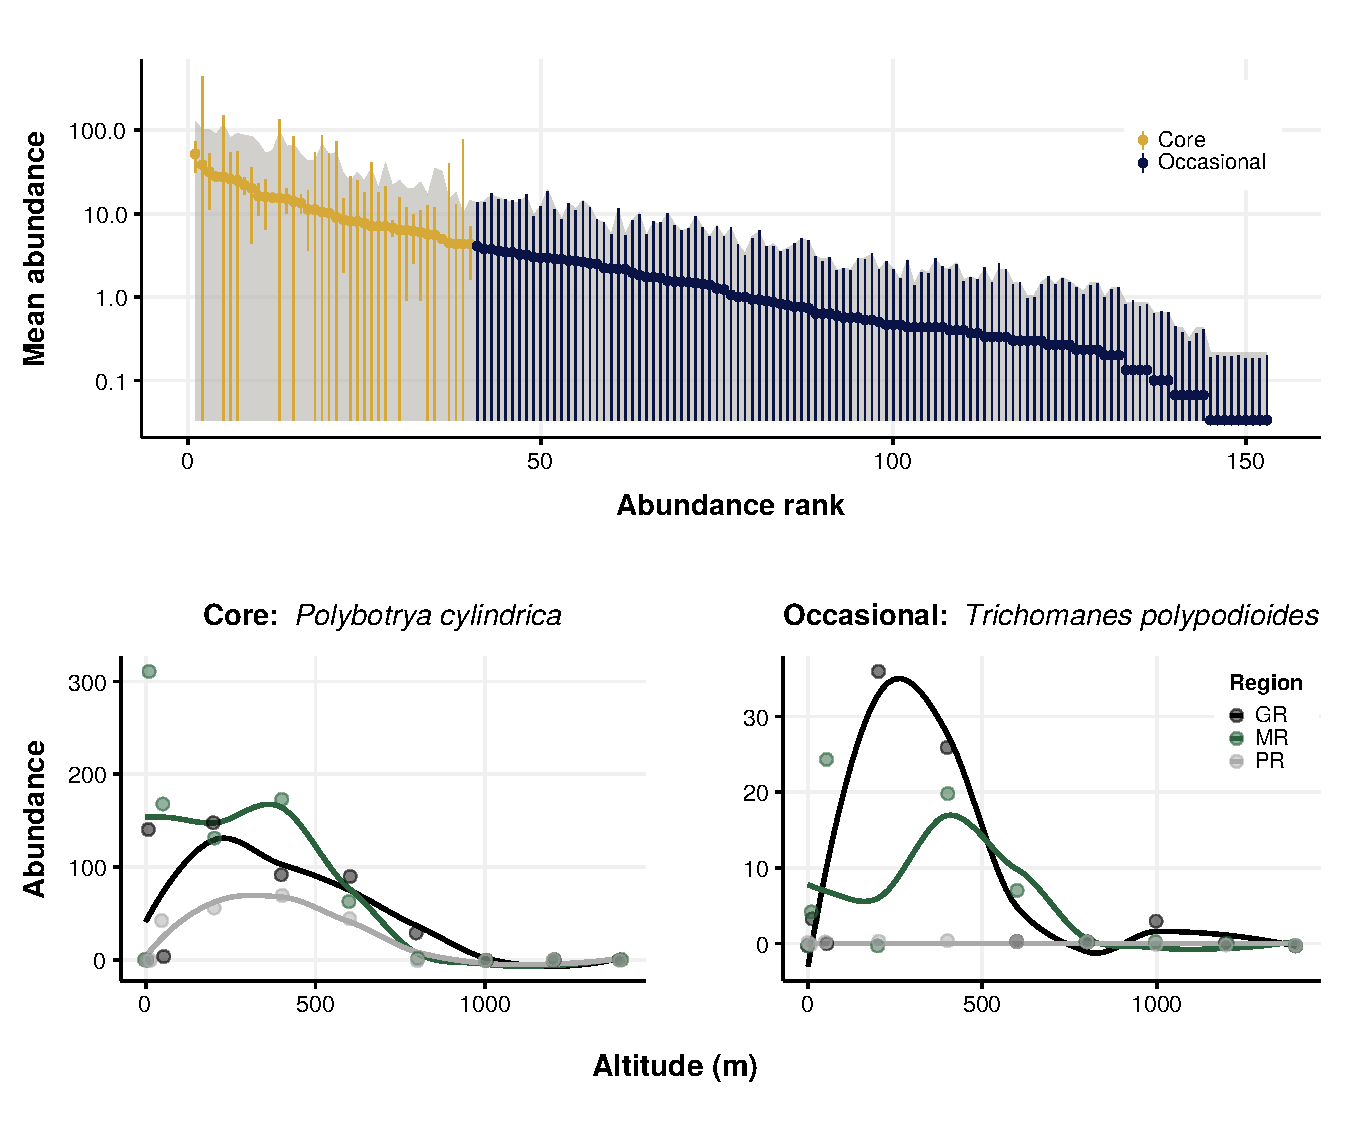
\includegraphics[scale=.48]{../figures/rad_mettacomunity.pdf}
\end{center}
\caption{\textbf{Upper panel:} Rank-abundance plot of the mean abudance of fern species across all sites $\pm$ one standard deviation (grey shadow). Vertical error bars show $\pm$ standard deviation of mean abundances predicted by dispersal limitation effects in our model (random effects $+$ intercept). Core species are ... and occasional species are ... . \textbf{Lower panels:} Examples of the variation of abundance along the altitudinal gradient of a core species (\emph{nome da espécie}, the most abundant among core species) , and a occasional species (\emph{nome da espécie}, the most abundant among occasionals). Points show recorded abundances and lines are \emph{lowess} splines in each of mountain range sampled (GR: Graciosa, MR: Marumbi, PR: Prata). Core species show a similar and unimodal variation of abundance in the three replicate regions. Abundances of occasional species does not show a consistent unimodal trend within or across mountain chains.}
\label{fig:radmeta}
\end{figure}


\newpage





\end{document}




